\documentclass[a4paper]{article}


\usepackage{alphabeta} 
\usepackage{enumitem} 
\usepackage{mathtools}
\usepackage{amsmath, amssymb} 
\usepackage{amsthm}
\usepackage{cancel} 
\usepackage[margin=0.70in]{geometry} 
\geometry{left=4.0cm,right=4.0cm,top=3cm,bottom=3cm}	%the page geometry as defined, A4=210x297mm
\usepackage{graphicx}
\usepackage{wrapfig}
\usepackage{caption}
\usepackage{textcomp}
\usepackage{tabto}
\usepackage{layout}
\usepackage{bm}
\usepackage{minipage-marginpar}
\usepackage[dvipsnames]{xcolor}
\usepackage{hyperref}
\usepackage{dutchcal}
\usepackage{derivative}
\usepackage{esint}
%\usepackage{biblatex}
\usepackage{subcaption}
\usepackage{booktabs}\usepackage{derivative}
\usepackage[flushleft]{threeparttable}

%%RENEW

\newtheorem{problem}{Άσκηση}
\newtheorem*{solution*}{Λύση}
\newtheorem{definition}{Ορισμός}[subsection]
\newtheorem{properties}{Ιδιότητες}[subsection]
\newtheorem{theorem}{Θεώρημα}[subsection]
\newtheorem{protash}{Πρόταση}[subsection]
\newtheorem{porisma}{Πόρισμα}[subsection]
\newtheorem{lemma}{Λήμμα}[subsection]
\newtheorem*{prooof}{Απόδειξη}
\newtheorem*{notes}{Παρατηρήσεις}
\newtheorem*{note}{Παρατήρηση}
\newtheorem*{app}{Εφαρμογή} 
\newtheorem*{example}{Παράδειγμα}
\newtheorem*{examples}{Παραδείγματα}

%\renewcommand{\labelenumi}{\roman{enumi}}
\newcommand{\approxtext}[1]{\ensuremath{\stackrel{\text{#1}}{\approx}}}
\renewcommand{\figurename}{Εικόνα.}
\renewcommand{\tablename}{Πίνακας.}
%\renewcommand\refname{New References Header}
\renewcommand*\contentsname{Περιεχόμενα}

\begin{document}
\begin{titlepage}			%makes a title page. Remember to change the author, CID, username and group number to what is appropriate for you!
	\centering
	{\scshape\LARGE Εθινικό Μετσόβιο Πολυτεχνείο\par}
	{\scshape \LARGE Σ.Ε.Μ.Φ.Ε.\par}
	\vspace{1cm}
	{\huge\bfseries Οπτική Φασματοσκοπία\par}
	\vspace{1cm}
	{\Large\itshape Θωμόπουλος Σπύρος\par}		%remember to change these!
	
	%		{\large Group \@group\unskip\strut\par}
	{\large A.M ge19042 \hfill \\}% spyros.thomop@gmail.com/ ge19042@mail.ntua.gr\par		%remember to change these!
	\vspace{1cm}
	{\large 20/10/2021\par}
\end{titlepage}


\newpage 
\section*{Σκοπός}
Ο στόχος της εν λόγω πειραματικής άσκησης είναι η μελέτη του φάσματος εκπομπής του υδρογόνου για την ορατή περιοχή (σειρά Balmer) και η εκτίμηση της σταθεράς Rydberg, με τη χρήση φασματοσκοπίου και λυχνίας ηλεκτρικής εκκένωσης υδρογόνου.

\section*{Θεωρητικά Στοιχεία}
 Από την επίλυση της εξίσωσης Schrodinger για το άτομο του Υδρογόνου θεωρώντας το πρωτόνιο ακίνητο προκύπτουν οι ενεργειακές στάθμες 
 $$E_{n} = \frac{m_e e^4 Z^2}{8\epsilon_{0} h^2 }\frac{1}{n^2} = -\frac{13.6}{n^2} eV$$
 Ακόμη έχουμε 
 
%\begin{align*}
 \begin{equation}\label{1}
 \Delta E = h v = h \frac{c}{\lambda} \Rightarrow  \\ 
 \frac{1}{\lambda} =\frac{m_e e^4 Z^2}{8 \epsilon_{0} h^3 c } \left( \frac{1}{n_{1}^2} -
 \frac{1}{n_{2}^2} \right)
 \end{equation}
%\end{align*}
 
Όπου ο αριθμός $ R = \frac{m_e e^4 Z^2}{8 \epsilon_{0} h^3 c }=1.097\times 10^{-7}m^{-1} $ είναι η σταθερά Rydberg.\newline \newline

Ως πηγή εκπομπής του φάσματος θα χρησιμοποιηθεί μία λυχνία ηλεκτρικής εκκένωσης υδρογόνου, η οποία εκπέμπει φως που περιέχει τα μήκη κύματος που αντισοιχούν στις παραπάνω ενεργειακές στάθμες.

Η μελέτη που γίνεται στην άσκηση περιορίζεται στη σειρά Balmer, δηλαδή για αποδιεγέρσεις που καταλήγουν στην ενεργειακή στάθμη $n_1 = 2$ και αντιστοιχούν σε εκπομπή φωτονίων με μήκος κύματος στην ορατή περιοχή του Η/Μ φάσματος. Εκμεταλλευόμενοι τις κυματικές ιδιότητες περίθλασης και διασποράς του φωτός θα υπολογίσουμε τα εν λόγω μήκη κύματος.

\subsubsection*{Περιγραφή οργάνων} 
Θα γίνει χρήση \textit{φασματοσκοπίου}, δηλαδή μίας συσκευής που καθιστά δυνατή την παρατήρηση της γωνιακής εκτροπής της κάθε συχνότητας εκπομπής με το μάτι. 
Θα χρησιμοποιηθούν δύο μέθοδοι με διαφορετικά φασματόμετρα: 
\footnote{Φασματόμετρο είναι αντίστοιχη συσκευή με το φασματοσκόπιο που μετρά ποσοτικά την ένταση της εκάστοστε συχνότητας.}
\begin{enumerate}


\item[i)] \underline{\textit{Φράγματος:}}
  Η φωτεινή δέσμη διέρχεται από ένα \textit{φράγμα διάδοσης}, το οποίο στην περίπτωσή μας είναι ένα πλακίδιο από διαφανές υλικό, αποτελούμενο από πολύ κοντινές χαραγές $\sim 300-600$ ανά $mm$. 
  
  Εξαιτίας του φαινομένου της περίθλασης, σε κάθε ένα από τα μήκη κύματος της φωτεινής δέσμης αντιστοιχεί μία διαφορετική γωνία ($\theta_n$) στην οποία συμβάλλει ενισχυτικά και εμφανίζονται μέγιστα σύμφωνα με την σχέση: 
\begin{equation}\label{2}
  dsin(\theta_n ) = m \lambda 
\end{equation}   
   όπου d είναι η απόσταση μετξύ δύο διαδοχικών χαραγών, άρα αν $N_0$ η συχνότητα χαραγών(χαραγές / μήκος), τότε $N_0 = 1/d$ και $m$ είναι ένας ακέραιος που δηλώνει την τάξη της περίθλασης . Πειραματικά θα μετρήσουμε τις γωνίες $\theta_n$ για τις πρώτες 3 τάξεις περίθλασης, $m=1,2,3$.
   
   
   
\item[ii)] \underline{\textit{Πρίσματος:}}
Η φωτεινή δέσμη διέρχεται από ένα γυάλινο πρίσμα. Λόγω του φαίνομένου της δισποράς η ταχύτητα της κάθε συχνότητας της δέσμης εντός του πρίσματος είναι διαφορετική και ως εκτουτου (n. Snell) διαθλάται σε διαφορετική γωνία. Άρα κάθε συχνότητα εξέρχεται απ' το πρίσμα σε διαφορετική γωνία, δηλαδή το φάσμα αναλύεται στα θεμελιώδη μήκη κύματος, τα οποία δεν αναλύονται περεταίρω. \\ 
Ορίζουμε ως \textit{γωνία εκτροπής} της κάθε συχνότητας την γωνία μεταξύ της πορείας της δέσμης αν δεν υπηρχε το πρίσμα και της τελικής πορείας με την παρουσία του πρίσματος. 

Η γωνία εκτροπής μεταβάλλεται καθώς αλλάζει η γωνία πρόσπτωσης και λαμβάνει ελάχιστο($D_{min}$), το οποίο μετράμε πειραματικά και υπολογίζουμε τον δείκτη διάθλασης: 
\begin{equation}\label{3}
  n= \frac{sin\left( (a+D_{min})/2 \right) }{sin(a/2)}
\end{equation}
με $a$ την γωνία της κορυφής του ισοσκελούς πρίσματος.
\end{enumerate}

\subsection*{Πειραματική διάταξη}
Η πειραματική διάταξη αποτελείται από: 
%\begin{minipage}[h!]{0.5\textwidth}\raggedright
\begin{itemize}
	\item Λυχνία Υδρογόνου
	\item Καταυθυντήρα, που έχει μία σχισμή για την ευθυγράμμιση της δέσμης και έναν φακό για την εστίασή της 
	\item Φράγμα / Πρίσμα 
	\item Γωνιομετρικό κύκλο (με ενσωματωμένο βερνιέρο για τις μετρήσεις των γωνιών) 
	\item Τηλεσκόπιο (με έναν φακό στο μπροστινό μέρος και έναν στο πίσω)
\end{itemize}
%\end{minipage}

\begin{figure}[h!]
	\centering
	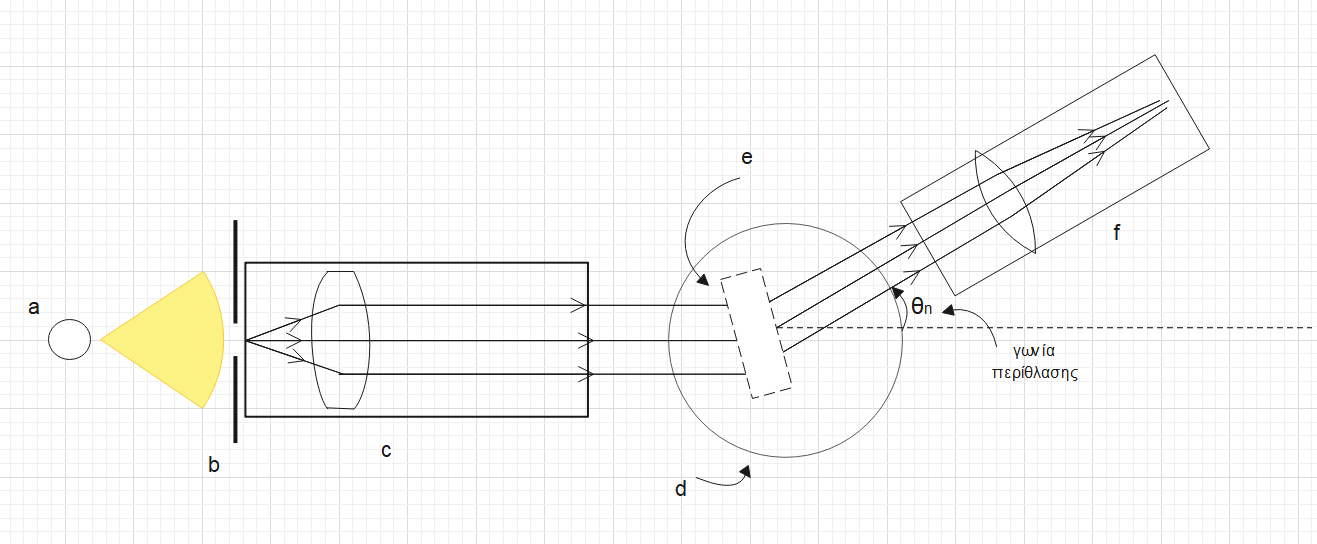
\includegraphics[scale=0.45]{setup.png}
	\caption{ a)Λάμπα Υδρογόνου, b) Λεπτή σχισμή, c) Κατευθυντήρας, d) Οπτική τράπεζα που περιστρέφεται. Στην βάση της υπάρχει ο γωνιομετρικός κύκλος, e) 1η μέθοδος: Φράγμα, 2η μέθοδος: Πρίσμα, f) τηλεσκόπιο}
\end{figure}

\subsection*{Πειραματική Διαδικασία - Επεξεργασία Μετρήσεων}
 
 **Σε όσους πίνακες χρησιμοποιηθούν, το κόκκινο χρώμα θα δηλώνει τιμές που έχουν μετρηθέι στο εργαστήριο.\\
 *** Οι πειραματικές τιμές του μήκους κύματος που δεν περιέχουν στα όρια του σφάλματός τους την αντίστοιχη θεωρητική τιμή σημειώνονται ως υπογραμμισμένες. \\ 

\subsubsection*{\textbf{\underline{(-) 1η Μέθοδος}(Φασματόμετρο Φράγματος)}}

Αρχικά βιδώνουμε την βάση του φράγματος στην οπτική τράπεζα και στερεώνουμε το φράγμα σε αυτήν με τις εγκοπές κάθετα στην τράπεζα.\footnote{Η συχνότητα χαραγών στο φράγμα είναι $N_0=300  \text{χαραγές } / mm$}
Έπειτα, ανοίγουμε το τροφοδοτικό, τοποθετούμε την λάμπα υδρογόνου ακριβώς πίσω από την σχισμή του κατευθυντήρα και ρυθμίζουμε τους φακούς του τηλεσκοπίου έτσι ώστε να φαίνεται καθαρά το είδωλο της σχισμής. 

Επειδή η γωνία περίθλασης της κάθε τάξης μετράται σε σχέση με την γωνία περίθλάσης μηδενικής τάξης ($m=0$), μετράμε την αντίστοιχη ένδειξη γι' αυτή τη γωνία: 
$$ \theta_0 = ( 340.1 \pm 0.1 ) ^{\circ} $$ 




Τώρα μετράμε τις υπόλοιπες φασματικές γραμμές, ξεκινώντας από τα δεξία. Αφού στρέψουμε το τηλεσκόπιο έτσι ώστε να φαίνεται η πρώτη γραμμή (κόκκινη) βιδώνουμε την αριστερή βίδα για να μην περιστρέφεται η οπτική τράπεζα και έπειτα με την δεξιά βίδα κουνάμε τον σταυρό εντός του τηλεσκοπίου μέχρι να ευθυγραμμιστεί με την φασματική γραμμή. 
\newline
Βλέπουμε εύκολα την ένδειξη του βερνιέρου για τη μονάδα την γωνίας, ενώ το δεκαδικό ψηφίο ταυτίζεται με τον αριθμό της πρώτης γραμμής του βεριέρου που πέφτει ακριβώς πάνω από μία γραμμή του γωνιομέτρου.
Επαναλαμβάνουμε τις μετρήσεις για τις φασματικές γραμμές των τριών πρώτων τάξεων περίθλασης. 
\footnote{Υπάρχει επικάλυψη των γραμμών των τάξεων, δηλαδη δεν εμφανίζονται πρώτα όλες οι γραμμές της τάξης n και έπειτα της n+1. Συγκεκριμένα για τις 3 πρώτες ισχύει: \newline 
Μπλε1$\rightarrow$Κυανούν1$\rightarrow$Κόκκινο1$\rightarrow$Μπλε2$\rightarrow$Κυανούν2$\rightarrow$Μπλε3
$\rightarrow$Κόκκινο2$\rightarrow$Κυανούν3$\rightarrow$Κυανούν4$\rightarrow$Μπλε4$\rightarrow$Κόκκινο3}
\newline

Συμπληρώνω τον παρακάτω πίνακα με χρήση της εξίσωσης (\ref{2}) για τον προσδιορισμό του πειραματικού μήκους κύματος, με $\theta_n$ να είναι η γωνιακή απόσταση μεταξύ του $\theta_0$ και της εκάστοτε μέτρησης\footnote{Για εύρεση του $\theta_m$: Αν η μέτρηση δεν ξεπερνάει τις $360^{ο}$ τότε απλώς αφαιρώ τις δύο γωνίες ενώ αν τις ξεπερνάει $\theta_m =( 360-\theta_0 + \text{ μετρούμενη γωνία}) = 19.9 + \text{ μετρούμενη γωνία}$.}
και $ d = 1/N_0 = 1/300 \cdot 10^{-3}m=3333.\bar{3} nm$

Ακόμη τα σφάλματα του κάθε μήκους κύματος όπως και της γωνίας $\theta_m$ προκύπτουν από διάδοση 
$$ \delta\theta_m = \sqrt{ \left(\pdv{\theta_m}{\theta_0}\delta\theta_0\right)^2 + \left(\pdv{\theta_m}{\theta}\delta\theta\right)^2} =
 	\sqrt{2}\delta\theta_0 = \sqrt{2}  0.1 = 0.1414 \simeq 0.1^{\circ}  $$% \simeq 0.0025 rad   $$  %\frac{\pi \cdot 0.1}{180} = 0.00 $$
 	
$$\delta\lambda=\sqrt{\left( \frac{\partial\lambda}{\partial\theta_m}\delta\theta_m\right)^2}= \left| \frac{d}{m}cos(\theta_m)\delta			\theta_m\right| \text{, ( το $\delta\theta_m$ είναι σε rad})$$

 	%δεν έχει νόημα τόσο μικρό σφάλμα, άρα το θέτω$ 0.1$

%\begin{tabular}{l|l|r|r} 
%	\hline
%	\multicolumn{2}{c}{Μετρ. Δεξιά} & \mulitcolumn{2}{c}{Μετρ. Αριστερά}  \\  %  \cline{1-4}  \\ \hline
%\multicolumn{2}{c|}{User B} &  \multicolumn{2}{c}{User C} \\
%	 \hline
%\multicolumn{2}{c}{Μετρ. Αριστερά}
% Τάξη &  Χρώμα &  Μετρ. Δεξιά &  Μετρ. Αριστερά \\ \hline\hline  
%&   Μωβ &            332.8 &               347.5 \\ 
%1  & Κυανούν &            331.9 &               348.2 \\ 
%&  Κόκκινο &            329.0 &               351.3 \\   \hline
% & Μωβ &            325.1 &               355.0 \\  
%2&  Κυανούν &            323.5 &               356.9 \\ 
%&  Κόκκινο &            317.2 &                 2.9 \\ \hline
%&  Μωβ &            317.6 &                 2.6 \\
%3&    Κυανούν &            314.8 &                 5.9 \\
%&     Κόκκινο &            304.5 &                15.8 \\	
%\end{tabular}

%\begin{flushleft}

\begin{table}[h]
\centering
\small
\caption{ }
\begin{tabular}{l|l|r|r|r|r|r|r|r|r}
%\hline
%\begin{tabularx}{\linewidth}{@{}XS[table-format=3.0]S[table-format=2.4]S[table-format=1.4]S[table-format=-1.4]S[table-format=2.4]@{}}
\toprule
\multicolumn{2}{c|}{} & \multicolumn{4}{c|}{Δεξιά} &  \multicolumn{4}{c}{Αριστερά} \\
	 \hline
m & Χρώμα &  θ($\pm0.1^{\circ}$)&  $\theta_n$($\pm0.1^{\circ}$) &  $sin(\theta_n)$ &  $\lambda_{exp}\pm\delta\lambda$ &  θ($pm0.1^{\circ}$)&  $\theta_n$($\pm0.1^{\circ}$) & $sin(\theta_n)$ &  $\lambda_{exp}\pm\delta\lambda$\\ 
 & & & & & $(nm)$ & & & & $(nm)$ \\ 
\hline \hline
& Μωβ 		&  \textcolor{red}{332.8} &         7.3 &        0.127 &    $423.6\pm 8.3$ & \textcolor{red}{347.5} &     7.4 &    0.128 &   $428.9\pm8.3$ \\
1& Κυανούν &  \textcolor{red}{331.9} &         8.2 &        0.142 &    $475.4\pm8.2$ & \textcolor{red}{348.2} &    8.1 &    0.140 &     $469.7\pm8.3$ \\
& Κόκκινο &  \textcolor{red}{329.0} &        11.1 &        0.192 &    $641.7\pm8.2$ & \textcolor{red}{351.3} &  11.2 &       0.194 &    $647.4\pm8.2$ \\   
\hline 
& Μωβ 		&  \textcolor{red}{325.1} &        15.0 &        0.258 &    $431.4\pm4.0$ & \textcolor{red}{355.0} & 14.9 &       0.257 &   $428.6\pm4.0$ \\
2& Κυανούν &  \textcolor{red}{323.5} &        16.6 &        0.285 &    $476.1\pm4.0$ & \textcolor{red}{356.9} & 16.8 &       0.289 &    $481.7\pm4.0$ \\
& Κόκκινο &  \textcolor{red}{317.2} &        22.9 &        0.389 &    $648.5\pm3.8$ &   \textcolor{red}{2.9} & 22.8 &       0.387 &     $645.9\pm3.8$ \\   
\hline
& Μωβ 		&  \textcolor{red}{317.6} &        22.5 &        0.382 &    $425.2\pm2.6$ &   \textcolor{red}{2.6} &  22.5 &      0.382 &   $425.2\pm2.6$ \\
3& Κυανούν &  \textcolor{red}{314.8} &        25.3 &        0.427 &    $474.8\pm2.5$ &   \textcolor{red}{5.9} &   25.8 &       0.435 &  $483.6\pm2.5$ \\
& Κόκκινο &  \textcolor{red}{304.5} &        35.6 &        0.582 &    $646.8\pm2.3$&  \textcolor{red}{15.8} &    35.7 &       0.583 &   $648.4\pm2.3$ \\
%\hline
\bottomrule
 %\end{tabularx}
\end{tabular}
\end{table}

%\begin{table}[h]
%\centering
%\small
%\caption{ }
%\begin{tabular}{l|l|r|r|r|r|r|r|r|r}
%%\hline
%%\begin{tabularx}{\linewidth}{@{}XS[table-format=3.0]S[table-format=2.4]S[table-format=1.4]S[table-format=-1.4]S[table-format=2.4]@{}}
%\toprule
%\multicolumn{2}{c|}{} & \multicolumn{4}{c|}{Δεξιά} &  \multicolumn{4}{c}{Αριστερά} \\
%	 \hline
%m & Χρώμα &  θ($\pm0.1^{\circ}$)&  $\theta_m$($\pm0.1^{\circ}$) &  $sin(\theta_m)$ &  $\lambda_{exp}$ &  θ($\pm0.1^{\circ}$)&  $\theta_m$($\pm0.1^{\circ}$) & $sin(\theta_m)$ &  $\lambda_{exp}$\\ 
% & & & & & $(nm)$ & & & & $(nm)$ \\ 
%\hline \hline
%& Μωβ 		&  \textcolor{red}{332.8} &         7.3 &        0.127 &    $423.6$ & \textcolor{red}{347.5} &     7.4 &    0.128 &   $428.9$ \\
%1& Κυανούν &  \textcolor{red}{331.9} &         8.2 &        0.142 &    $475.4$ & \textcolor{red}{348.2} &    8.1 &    0.140 &     $469.7$ \\
%& Κόκκινο &  \textcolor{red}{329.0} &        11.1 &        0.192 &    $641.7$ & \textcolor{red}{351.3} &  11.2 &       0.194 &    $647.4$ \\   
%\hline 
%& Μωβ 		&  \textcolor{red}{325.1} &        15.0 &        0.258 &    $431.4$ & \textcolor{red}{355.0} & 14.9 &       0.257 &   $428.6$ \\
%2& Κυανούν &  \textcolor{red}{323.5} &        16.6 &        0.285 &    $476.1$ & \textcolor{red}{356.9} & 16.8 &       0.289 &    $481.7$ \\
%& Κόκκινο &  \textcolor{red}{317.2} &        22.9 &        0.389 &    $648.5$ &   \textcolor{red}{2.9} & 22.8 &       0.387 &     $645.9$ \\   
%\hline
%& Μωβ 		&  \textcolor{red}{317.6} &        22.5 &        0.382 &    $425.2$ &   \textcolor{red}{2.6} &  22.5 &      0.382 &   $425.2$ \\
%3& Κυανούν &  \textcolor{red}{314.8} &        25.3 &        0.427 &    $474.8$ &   \textcolor{red}{5.9} &   25.8 &       0.435 &  $483.6$ \\
%& Κόκκινο &  \textcolor{red}{304.5} &        35.6 &        0.582 &    $646.8$&  \textcolor{red}{15.8} &    35.7 &       0.583 &   $648.4$ \\
%%\hline
%\bottomrule
% %\end{tabularx}
%\end{tabular}
%\end{table}

 %\end{flushleft}
% \newline \newline

% \end{flushleft} 

Πρέπει να σημειωθεί πως οι φσαματικές γραμμές των διαφόρων τάξεων αλληλεπτικαλύπτονται στα πλαίσια του σφάλματός τους.

\newpage 

Οι πειραματικές μέσες τιμές για κάθε μήκος κύματος και οι αντίστοιχες θεωρητικές συγκεντρώνονται στον παρακάτω πίνακα:\footnotemark:
\footnotetext{Οι μέσες τιμές και τα αντίστοιχα σφάλματα προκύπτουν από τις σχέσεις: 
a)$\overline{\lambda} = \frac{1}{6}\sum_{i=1}^{6}\lambda_i$ και
%\textcolor{orange}{
 b) $\delta\lambda = \left( \frac{\sum_{i=1}^{6}(\lambda_i-\overline{\lambda})^2}{6\cdot 5}\right)^{1/2} $}
 %}
 
 \begin{table}[h!]
\centering
\caption{ }
	\begin{tabular}{c|c|c}
	Χρώμα & $\overline{\lambda}_{πειρ}(nm)$ & $\lambda_{θεωρ}(nm)$  \\
	\hline \hline 
	Μωβ      & \underline{$427.2 \pm 2.7$} & 434.1 \\ 
	Κυανούν  & \underline{$476.8 \pm 4.6$} & 486.1 \\ 
	Κόκικινο & \underline{$646.5 \pm 2.3$} & 656.3 \\  
	\end{tabular}	 
 
 \end{table}
 
%\begin{itemize}
%\item[.] $\overline{\lambda}^{πειρ}_{κοκ } = ( 646.5 \pm 1.0) nm $ 
%\item[.] $\overline{\lambda}^{πειρ}_{κυαν} = ( 476.8 \pm 2.1) nm $ 
%\item[.] $\overline{\lambda}^{πειρ}_{μωβ } = ( 427.2 \pm 1.2) nm $ 
%\hline
%\item[.] $\overline{\lambda}^{πειρ}_{κοκ1 } = ( 644.0 \pm ) nm $ 
%\item[.] $\overline{\lambda}^{πειρ}_{κυαν1} = ( 472.1 \pm ) nm $ 
%\item[.] $\overline{\lambda}^{πειρ}_{μωβ1 } = ( 426.0 \pm ) nm $ 
%\item[.] $\overline{\lambda}^{πειρ}_{κοκ2 } = ( 646.6 \pm ) nm $ 
%\item[.] $\overline{\lambda}^{πειρ}_{κυαν2} = ( 478.5 \pm ) nm $ 
%\item[.] $\overline{\lambda}^{πειρ}_{μωβ2 } = ( 429.5 \pm ) nm $ 
%\item[.] $\overline{\lambda}^{πειρ}_{κοκ3 } = ( 647.0 \pm ) nm $ 
%\item[.] $\overline{\lambda}^{πειρ}_{κυαν3} = ( 454.0 \pm ) nm $ 
%\item[.] $\overline{\lambda}^{πειρ}_{μωβ3 } = ( 424.8 \pm ) nm $
%\end{itemize}

%Οι θεωρητικές τιμές για τα μήκη κύματος είναι $\lambda_{ερ}=656.3nm$, $\lambda_{κυαν}=486.1nm$, $\lambda_{μωβ1}=434.1nm$, %\textcolor{orange}{$\lambda_{μωβ2}=410.2nm$}

Παρατηρώ ότι οι θεωρητικές τιμές δεν ανήκουν στο διάστημα του σφάλματος που βρέθηκε για τις πειραματικές τιμές,
% πράγμα που σημαίνει πως υπήρχαν αστοχίες κατά την πειραματική διαδικασία,
 παρ'ολο που τα σχετικά σφάλματα είναι μικρότερα από $1\%$. Αυτό σημαίνει πως έχουμε μικρή ακρίβεια αλλά μεγάλη αξιοπιστία. Ενδεχομένως η απόκλιση αυτή να οφείλεται κυρίως στο γεγονός ότι το φράγμα περίθλασης δεν ήταν ακριβώς κάθετο στην φωτεινή δέσμη. 
Αυτό αλλάζει την σχέση (\ref{2}) σε $d(sin(\phi) + sin(\theta_m))=m\lambda$, όπου $\phi$ η γωνία πρόσπτωσης.\footnote{https://opencourses.uoc.gr/courses/course/view.php?id=357} Γίνεται έτσι εμφανής η επίδραση αυτής της παραμέτρου στα αποτελέσματα.
%Ακόμη, ίσως να υπήρξε αλλοίωση των μετρήσεων εξαιτίας της ύπαρξης φωτισμού στο εργστήριο κατά %την διάρκεια των μετρήσεων ή/και της εισχώρησης αέρα εντός της λυχνίας από την πολυκαιρία.
\\ 
Για τον υπολογισμό της σταθεράς Rydberg από την σχέση (\ref{1}) έχουμε: 
$$ R_{i} = \frac{1}{\lambda_i} \frac{1}{1/4 - 1/n_2^2} \text{ ,i=\{κόκ, κυαν, μωβ\}} \footnotemark$$
\footnotetext{όπου $n_2=3,4,5 $ για κόκκινο, κυανό και μωβ αντίστοιχα }
απ' όπου προκύπτει $R_{κοκ}=1.113$, $R_{κυαν}=1.118$, $R_{μωβ}=1.115$, με μονάδες $10^{-7}m^{-1}$. 
Άρα η αντίστοιχη μέση τιμή και το σφάλμα της είναι: 
$$ \overline{R} = (1.12 \pm 0.01) \times 10^{-7}m^{-1}$$

Παρατηρώ πως η πειραματικλή τιμή δεν περιλαμβάνει στα όρια του σφάλματός της την θεωρητική, παρ'όλο που έιναι σχετικά κοντά σε αυτή, απέχει περίπου $2\%$ της τιμής της.

\subsubsection*{\textbf{\underline{(-) 2η Μέθοδος}(Φασματόμετρο Πρίσματος)}}
Τώρα αφαιρούμε το φράγμα, ξεβιδώνουμε την βάση του, τοποθετούμε το πρίσμα\footnotemark  στην οπτικη τράπεζα και παρατηρούμε τις γραμμές του φάσματος με γυμνό μάτι. Τώρα περιστρέφοντας την οπτική τράπεζα (αλλάζοντας δηλαδή την γωνία πρόσπτωσης της δέσμης στο πρίσμα) παρατηρούμε ότι το φάσμα κινείται και καθώς συνεχίζουμε αυτή τη διαδικασία βλέπουμε πως κάποια στιγμή η κατεύθυνση της κίνησης αλλάζει. Αυτό σημαίνει ότι σε εκείνη την περιοχή βρίσκονται οι ελάχιστες γωνίες εκτροπής για το κάθε μήκος κύματος. 

Για να προσδιορίσουμε με ακρίβεια αυτή τη γωνία επαναλαμβάνουμε την παρακάτω διαδικασία και για τα τρία χρώματα(κόκκινο, κυανούν, μωβ): 

\footnotetext{Το πρίσμα είναι ισοσκελές με γωνία κορυφής $a=60^{\circ}$.}



Φέρνουμε διαρκώς το τηλεσκόπιο σε θέση τέτοια ώστε να φαίνεται το υπό μελέτη χρώμα. Περιστρέφουμε την οπτική τράπεζα μέχρι να βρουμε το σημείο στο οποίο αλλάζει η κατεύθυνση της κίνησης του χρώματος όπου και την ακινητοποιούμε. Αφού ευθυγραμμίσουμε τον σταυρό εντός του τηλεσκοπίου με την υπό μελέτη φασματική γραμμή, μετράμε την ένδειξη του βερνιέρου (γωνία $\phi_1 $) και έπειτα μετράμε την γωνία που θα ακολουθούσε η φωτεινή δέσμη αν δεν υπήρχε το πρίσμα (γωνία $\phi_0$, στην οποία φαίνεται το είδωλο της σχισμής).

Η απόσταση των δύο αυτών γωνιών είναι η γωνία ελάχιστης εκτροπής του υπό μελέτη μήκους κύματος.
 
\begin{figure}[h!]\label{fig2}
\centering  
\caption{ }
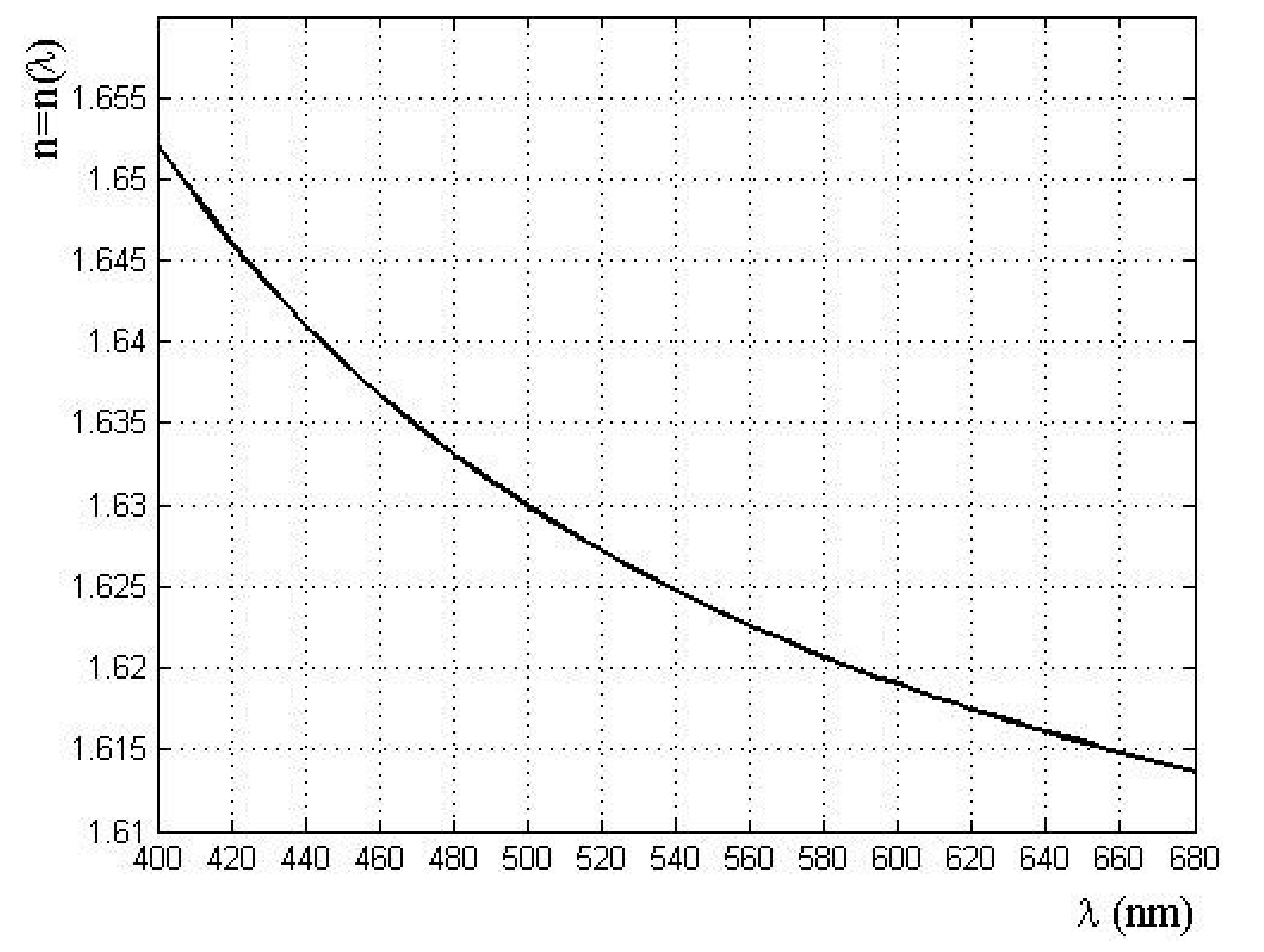
\includegraphics[scale=0.35]{n.png}
\end{figure}
Με τον παραπάνω τρόπο, την σχέση (\ref{3}) για τον υπολογισμό του δείκτη διάθλασης και την καμπύλη (Εικόνα. 2) που δίνει τον δέικτη διάθλασης του γυαλιού συναρτήσει του μήκους κύματος για τον προσδιορισμό του μήκους κύματος, συμπληρώνουμε τον παρακάτω πίνακα: 
\newline

\begin{table}[h!]
\centering 
\caption{ }
\begin{tabular}{l|r|r|r|r|r|r} 
  Χρώμα & $\lambda_{θεωρ}(nm)$&$\phi_1 (\pm0.1^{\circ})$ & $\phi_0 (\pm0.1^{\circ})$ &   $D_{min}(\pm0.1^{\circ})$
   & n & $\lambda_{πειρ}(nm)$ \\  
\hline \hline  
 Κόκκνο &   656.3 & \textcolor{red}{28.0} & \textcolor{red}{340.2} &   47.8   & $1.616\pm 0.106$   & $650\pm10$ \\     %598
  Κυανούν &   486.1 & \textcolor{red}{28.7} & \textcolor{red}{339.6} &   49.1 & $1.629\pm 0.095$   & \underline{$500\pm10$} \\     %9244
  Μωβ &   434.1 & \textcolor{red}{29.1} & \textcolor{red}{338.8} &   50.3     & $1.641\pm 0.085$   & \underline{$445\pm10$} \\     %1302
 \end{tabular}
 \end{table}
 
 
 
 
Το σφάλμα για την $D_{min}$ και τον δείκτη διάθλασης $n$ προκύπτουν από διάδοση σφαλμάτων ως εξής: 
$$ \delta D_{min} = \sqrt{\left( \pdv{D_{min}}{\phi_0}\delta\phi_0\right)^2 + \left( \pdv{D_{min}}{\phi_1}\delta\phi_1 \right)^2 } = 
						\sqrt{1\cdot\delta\phi_0^2 + 1\cdot\delta\phi_1^2} = 0.1\sqrt{2} \simeq 0.1414 \simeq 0.1$$ 
$$ \delta n       = \sqrt{  \left( \pdv{n}{D_{min}} \delta D_{min} \right) ^2 } = 
					\left| \frac{1}{2}\frac{cos\left((a+D_{min})/2\right)}{sin(a/2)}\right|	= \left| cos(30+D_{min}/2) \right|\footnotemark $$ \footnotetext{$\delta n_{κοκ} \simeq 0.106\simeq 0.1$, $\delta n_{κυαν} \simeq 0.0949 \simeq 0.1 $,
					$\delta n_{μωβ} \simeq 0.0845 \simeq 0.1$} 
					
Οι θεωρητικές τιμές για τα μήκη κύματος είναι $\lambda_{ερ}=656.3nm$, $\lambda_{κυαν}=486.1nm$, $\lambda_{μωβ1}=434.1nm$, %.\textcolor{orange}{$\lambda_{μωβ2}=410.2nm$}. 
Παρατηρώ ότι 2 από τις 3 τιμές των μηκών κύματος δεν συμπίπτουν με τις θεωρητικές, χωρίς ωστόσο το όριο του σφάλματος να απέχει πολύ από αυτές. 
Αυτό σημαίνει ότι υπάρχουν κάποια σφάλματα που ίσως δεν έχουν συμπεριληφθεί.
%, όπως το σφάλμα προσδιορισμού του σημείου αναστροφής της κίνησης του φάσματος.


Τα εν λόγω σφάλματα σχετίζονται ταυτόχρονα και με τα δύο μέρη της πειραματικής διαδικασίας και ενδεχομένως να επηρέασαν την ακρίβεια των αποτελεσμάτων. Παρατηρήθηκε ότι υπάρχει συστηματικό σφάλμα παράλαξης στο προσοφθάλμιο, δηλαδή η θέση του σταυρού εντός του τηλεσκοπίου εξαρτάται από την γωνία θέασης μέσω του προσοφθαλμίου.
%, όμως να γνωρίζουμε το πάχος της γραμμής και σε ποίες μετρήσεις υπήρξε η λάθος θέαση απ' το %τηλεσκόπιο δεν μπορούμε να βγάλουμε συμπέρασμα για την τάξη αυτών των σφαλμάτων.
Επιπλέον, ίσως να αλλοιώθηκαν οι μετρήσεις
εξαιτίας της ύπαρξης φωτισμού στο εργαστήριο κατά την διάρκεια των μετρήσεων ή/και εξαιτίας της εισχώρησης αέρα εντός της λυχνίας από την πολυκαιρία.

\subsection*{Συμπεράσματα}
Συνολικά τα αποτελέσματα ήταν σχετικά κοντά στα θεωρητικώς αναμενόμενα, χωρίς ωστόσο να τα περιέχουν στο διάστημα των σφαλμάτων τους. Οι παράγοντες που είχαν επίδραση κατά σειρά σημαντικότητας, εκτιμώ πως ήταν οι εξής: 
  το σφάλμα παράλλαξης στο προσοφθάλμιο,
%  η απόκλιση από την καθετότητα της τοποθέτησης του φράγματος από την φωτεινή δέσμη,
  η μη κάθετη τοποθέτηση του φράγματος στην φωτεινή δέσμη,
  η ύπαρξη φωτισμού στο εργαστήριο και 
  η πολυκαιρία της λυχνίας.

Για να βελτιώσουμε την ακρίβεια της μέτρησης της 1ης μεθόδου θα μπορούσαμε να αυξήσουμε την διακριτική ικανότητα του περιθλαστικού φράγματος, πράγμα που επιτυγχάνεται με την αντικατάσταση του φράγματος με ένα άλλο, το οποίο να έχει περισσότερες σχισμές $/mm$ και τότε θα διακρίνονται καλύτερα φασματικές γραμμές με γειτονικά μήκη κύματος.

Τέλος, αν τα συστηματικά σφάλματα που έχουν αναφερθεί περιορίζονταν, τότε σίγουρα η πρώτη μέθοδος είναι πιό αποτελεσματική, καθώς έχει μεγαλύτερη αξιοπιστία (precision) από την δεύτερη. Το συμπέρασμα με βάση τις δεδομένες μετρήσεις είναι το ίδιο, καθώς γενικά, δεδομένου ότι οι θεωρητικές τιμές δεν περιέχονται στο όριο του σφάλματος των πειραματικών, η επι τοις εκατό απόκλιση των πειραματικών απ' τις θεωρητικές είναι ελαφρώς μικρότρες με την πρώτη μέθοδο 
	
\begin{table}[h!]
\centering 
\begin{tabular}{c|c|c}
Χρώμα    & $\delta\lambda / \lambda \%$     & $\delta\lambda / \lambda \%$ \\ 
         &  1η Μέθοδος 						& 2η Μέθοδος 					\\ 
        \hline \hline
Κόκκινο  & 		2.1                           & 1.0 \\
Κυανούν  &  2.0 & 2.8 \\ 
Μωβ      & 1.6 & 2.5 
\end{tabular}
\end{table}


\end{document}
